\chapter{网站效果展示}

本章将主要展示已经部署上线的网站UI, 以及相应的资源发布、下载、查找的简明步骤, 以期读者能够通过对本章的阅读迅速掌握网站的使用方法。

\section{网站的用户界面}

用户首页, 有聊天盒、推荐种子等功能。左侧的一栏图标代表资源搜索下载、上传等细分功能。

\begin{figure}[h]
    \centering
    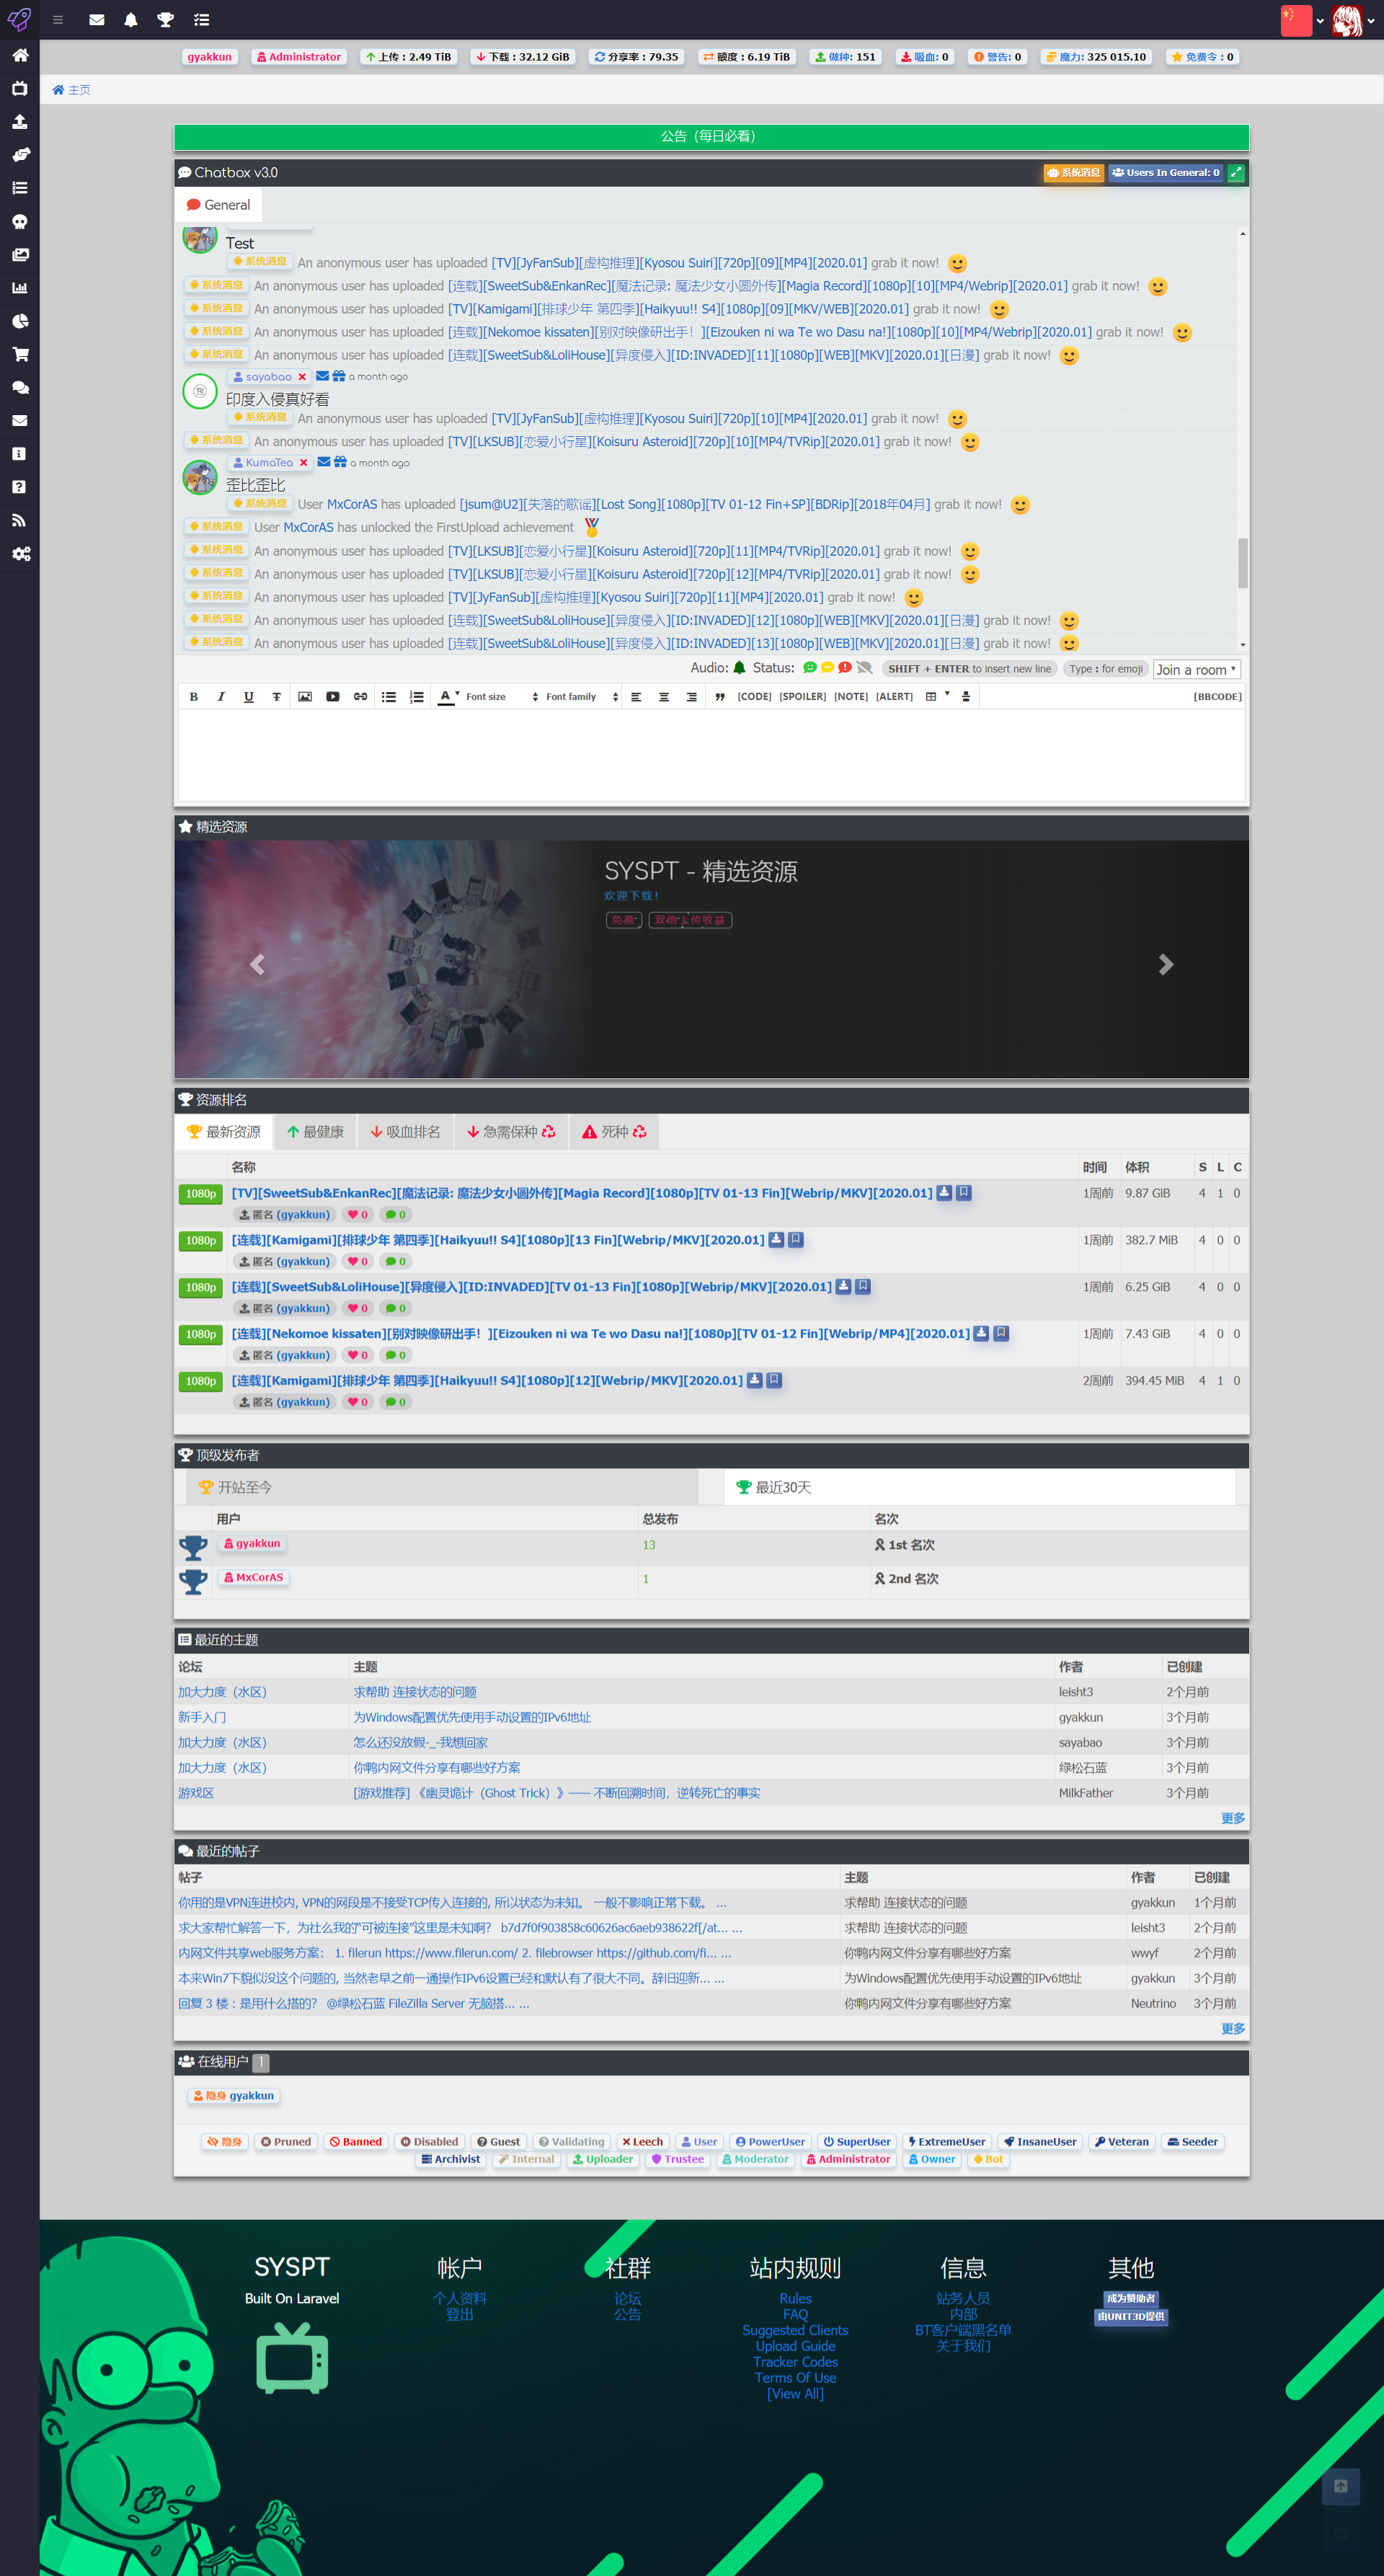
\includegraphics[width=0.45\textwidth]{support-files/5.1-index-ui.png}
    \caption{首页}
    \label{fig:webindex}
\end{figure}

\section{资源的查找与下载}

点击左侧的"资源"图标, 进入搜索页。在搜索框内输入关键字, 无需点按搜索按钮, 马上自动响应发起搜索请求。

\begin{figure}[h]
    \centering
    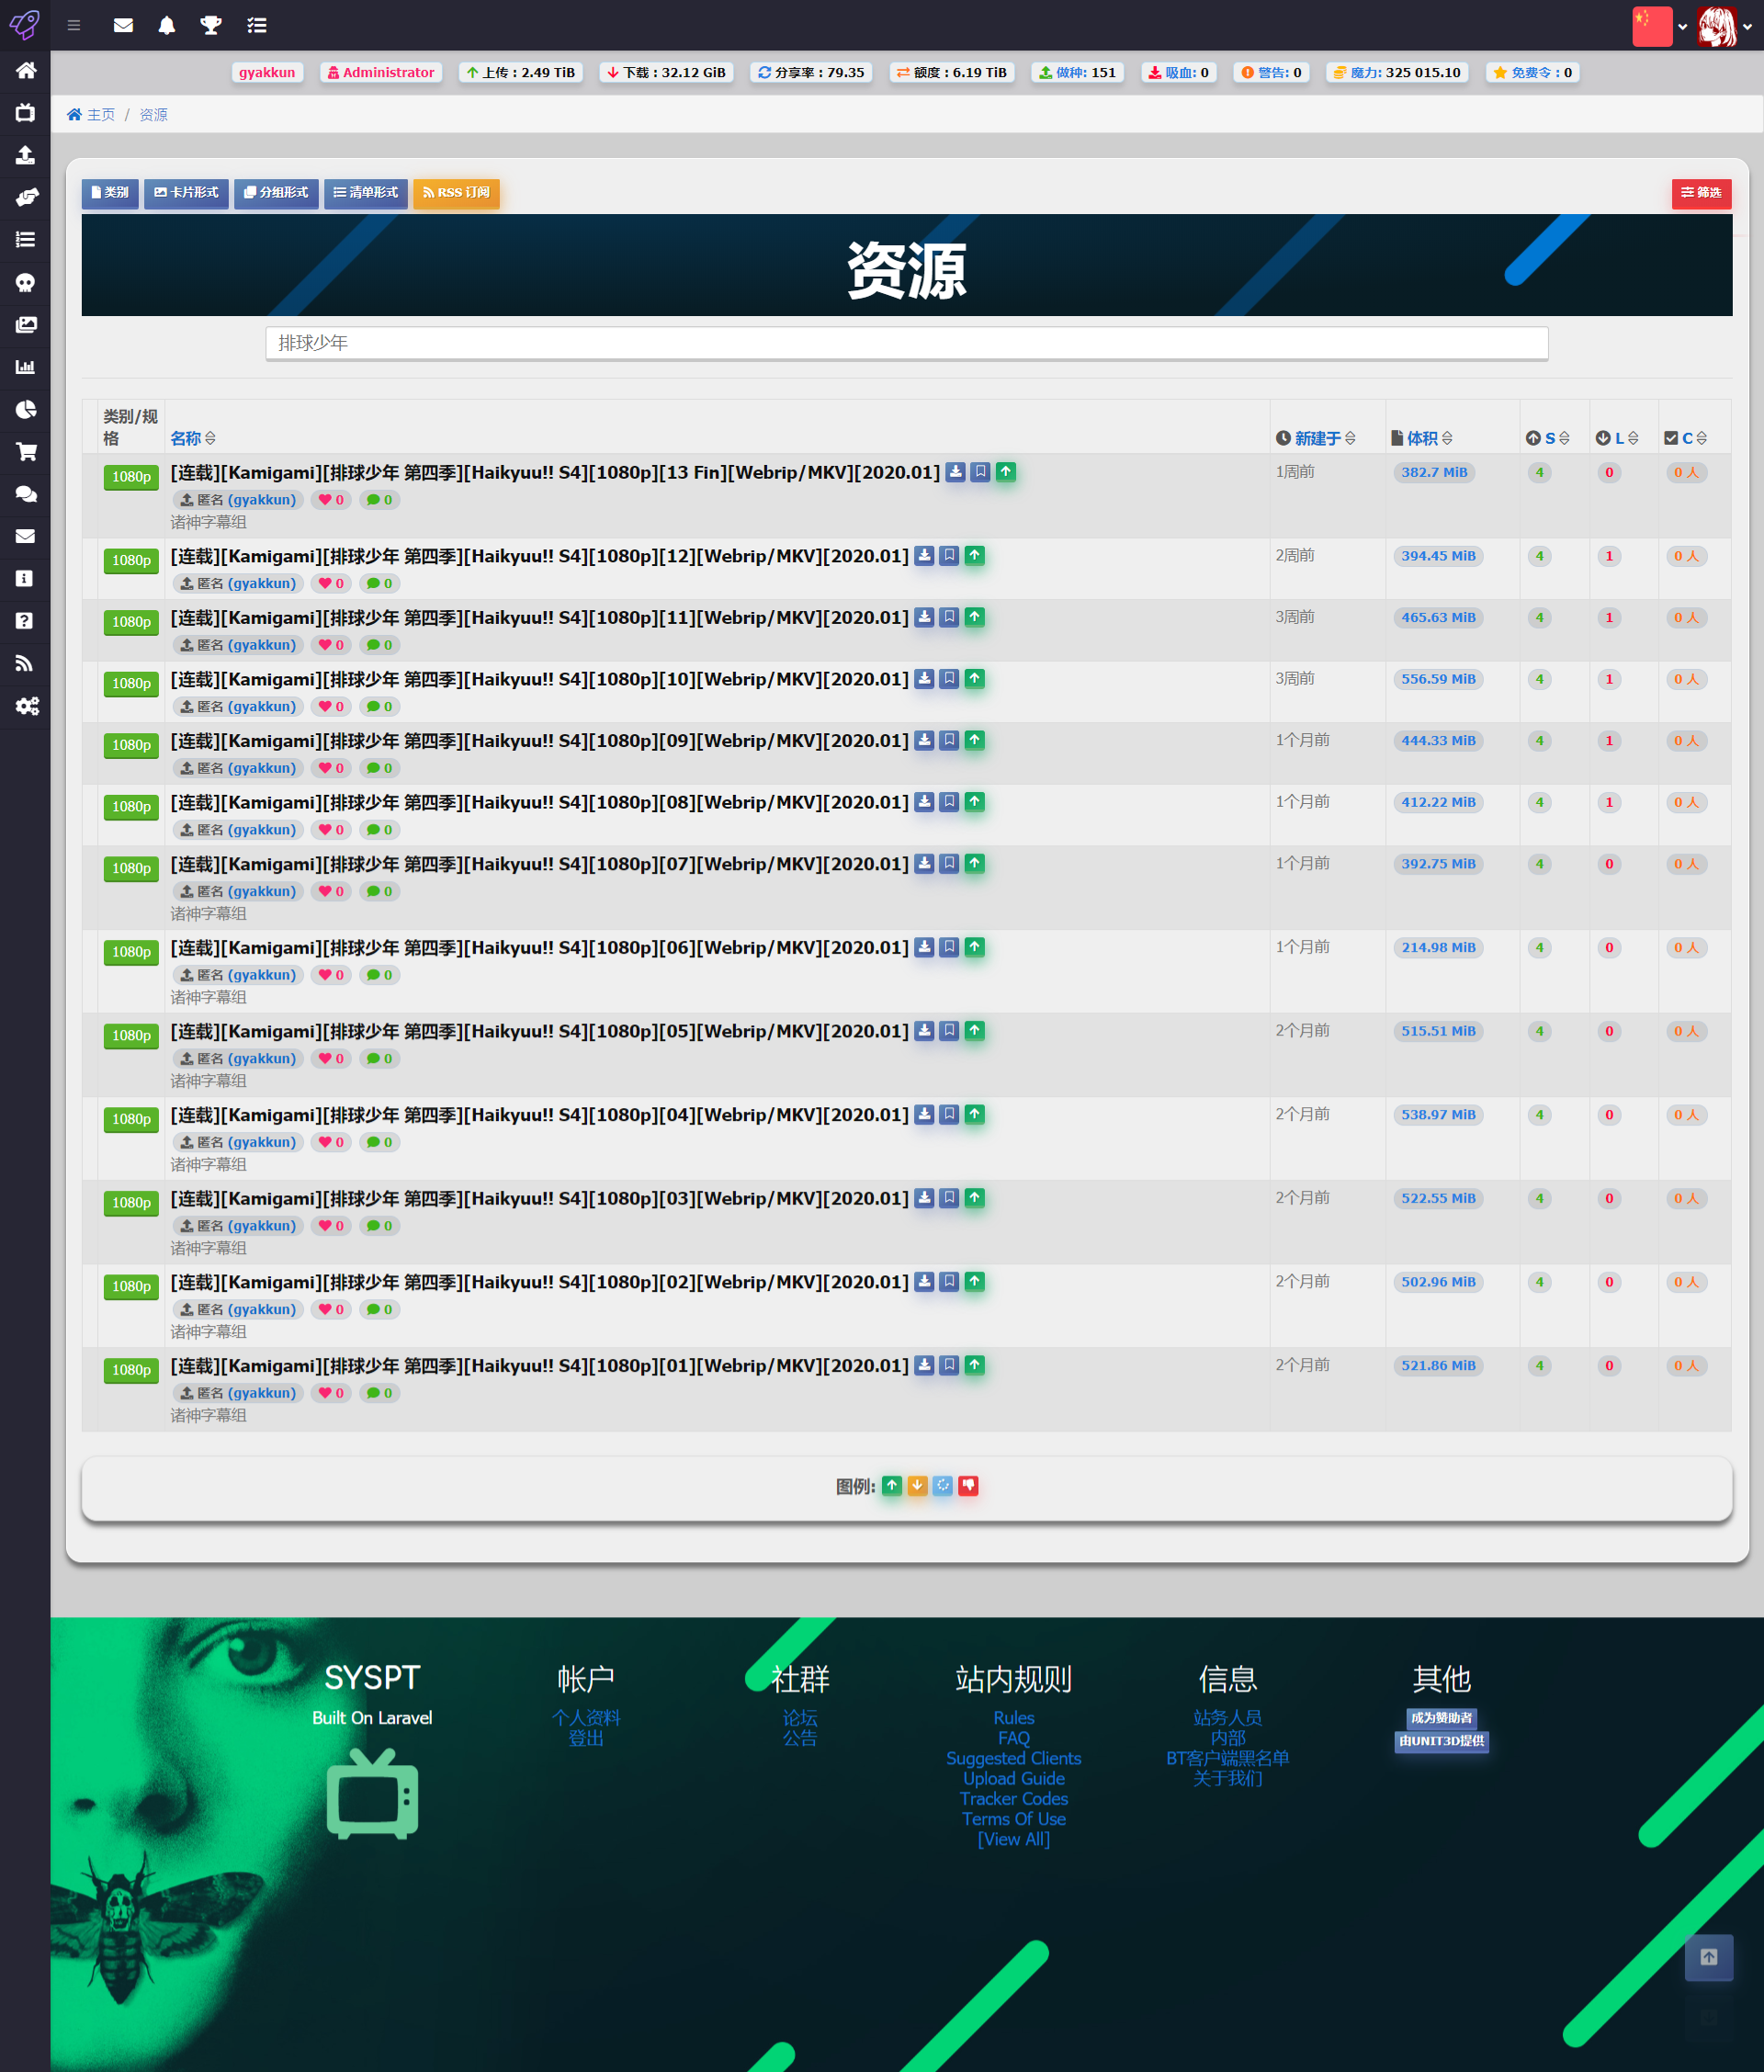
\includegraphics[width=0.65\textwidth]{support-files/5.2-search-page-1.png}
    \caption{简单搜索页}
    \label{fig:websearchpage1}
\end{figure}

如对搜索结果不满意, 或是要进行进一步的筛选, 可使用右上角的筛选器按钮, 进行高级搜素。

\begin{figure}[h]
    \centering
    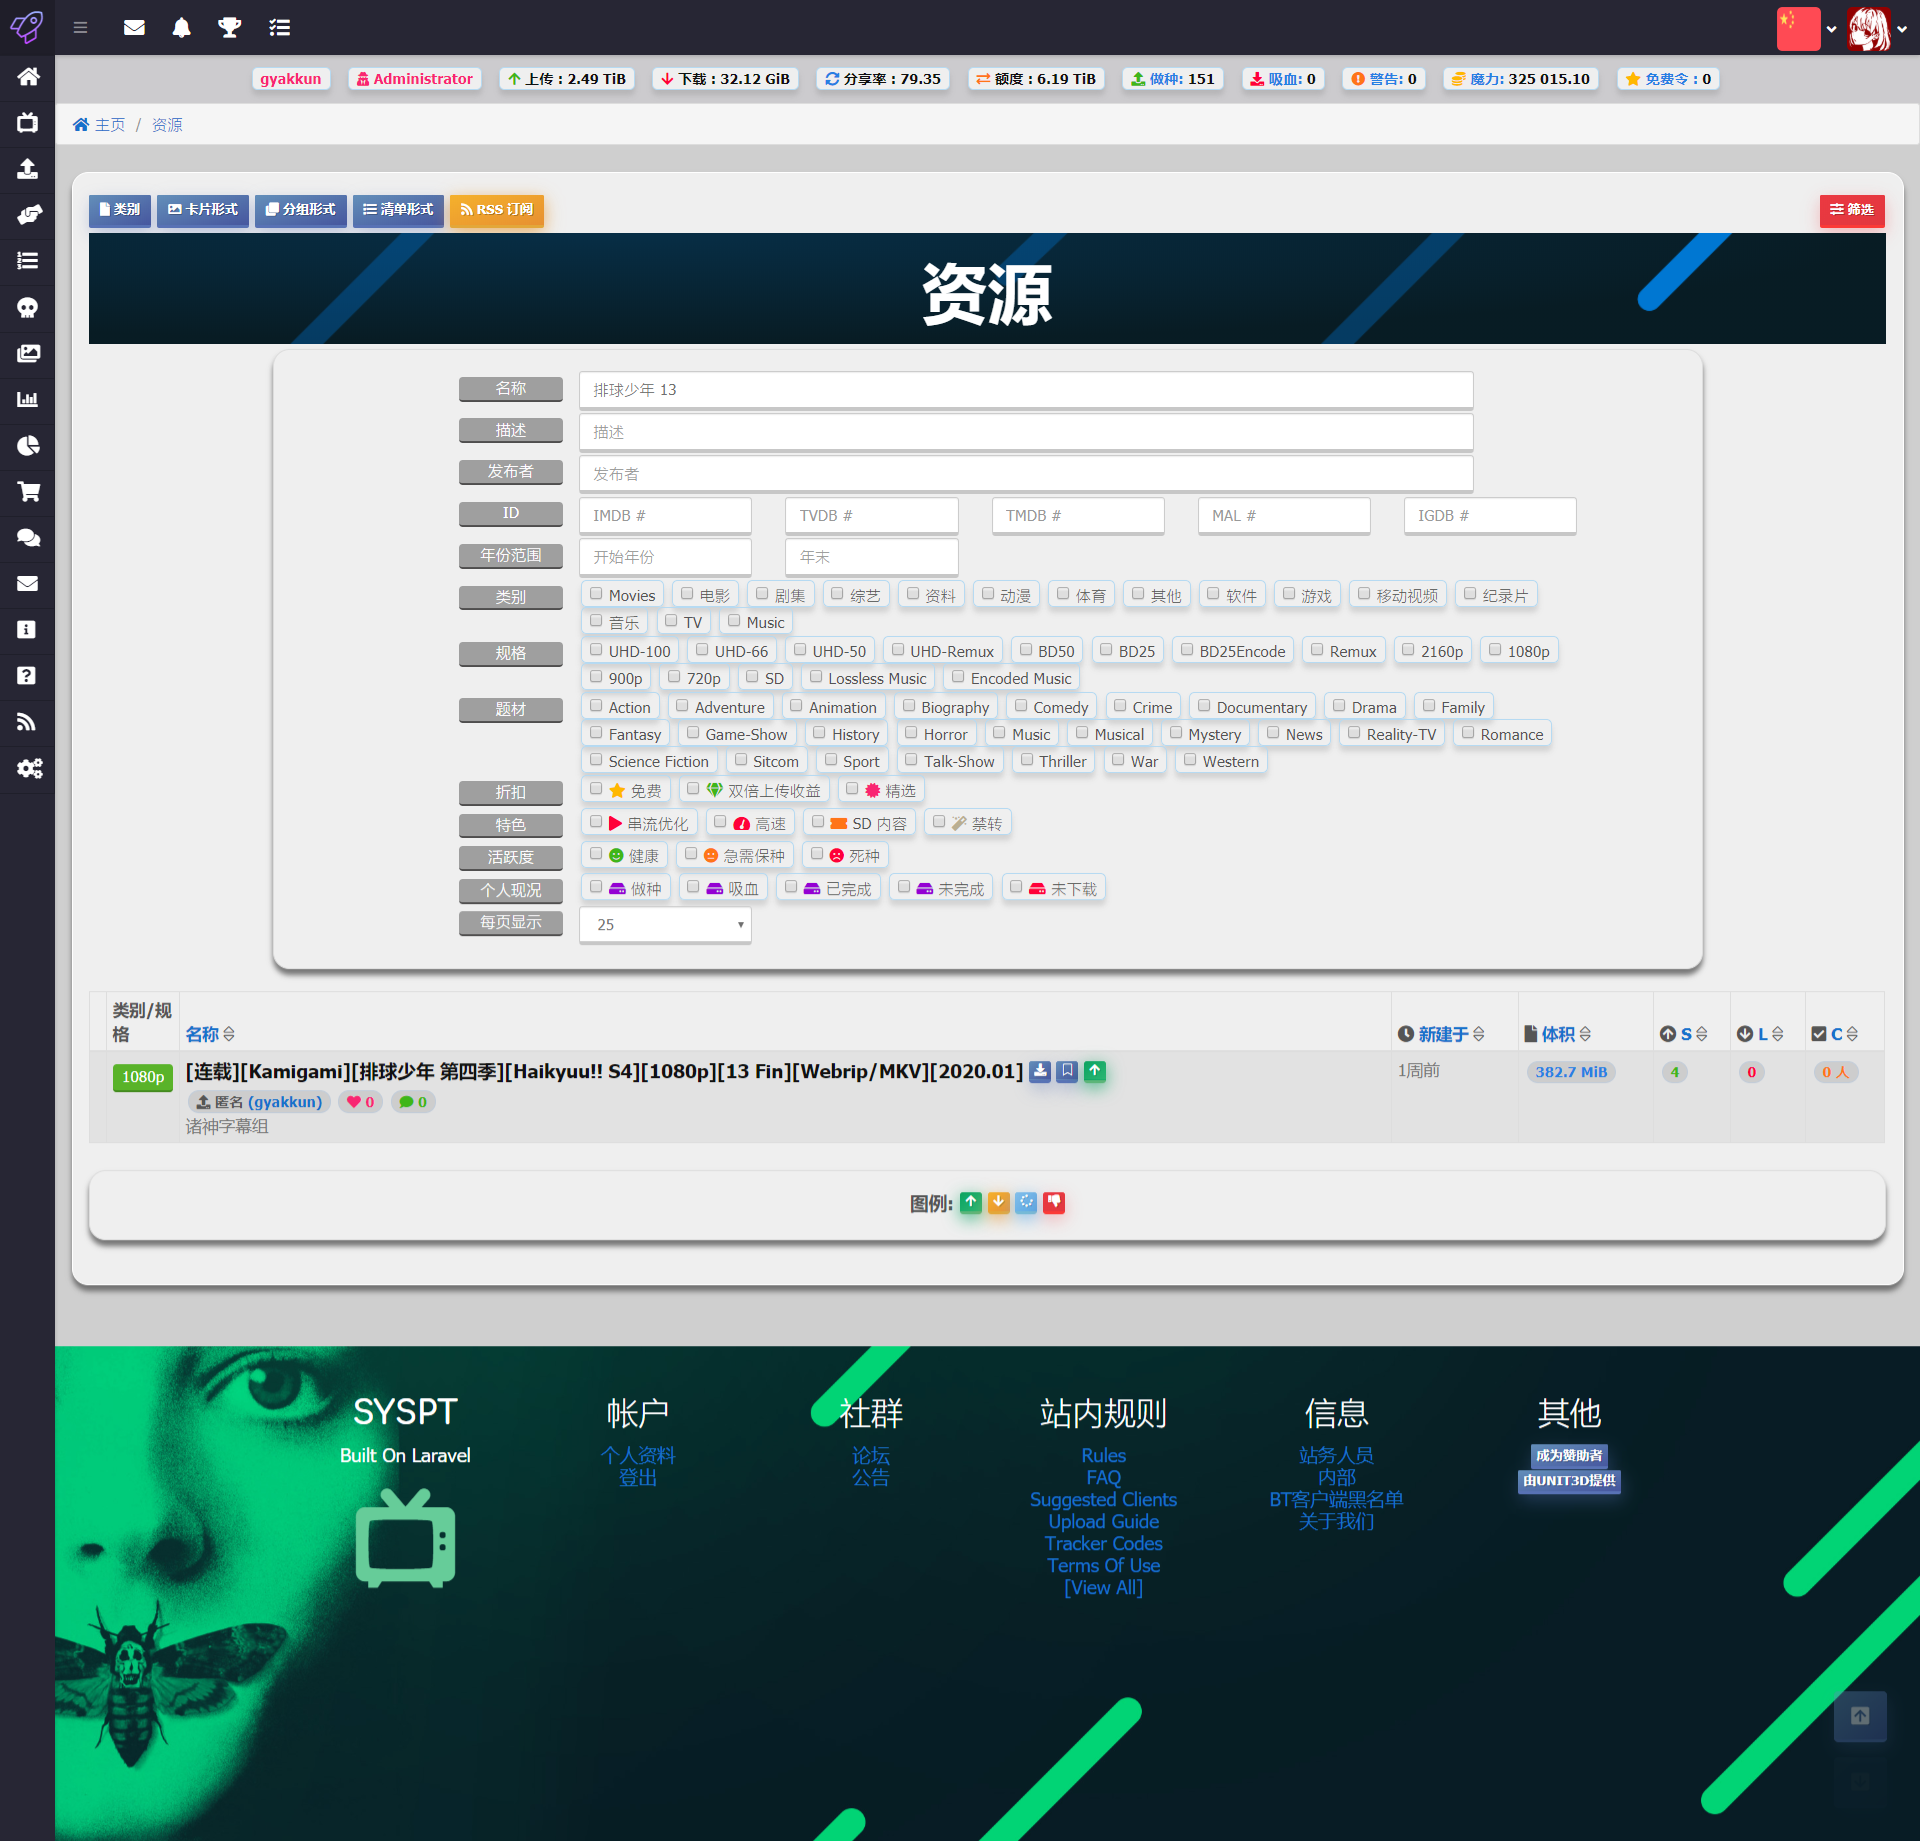
\includegraphics[width=0.9\textwidth]{support-files/5.2-search-page-2.png}
    \caption{高级搜索页}
    \label{fig:websearchpage2}
\end{figure}

在搜索结果列表点击想要下载的资源, 进入种子详情页面。

\begin{figure}[h]
    \centering
    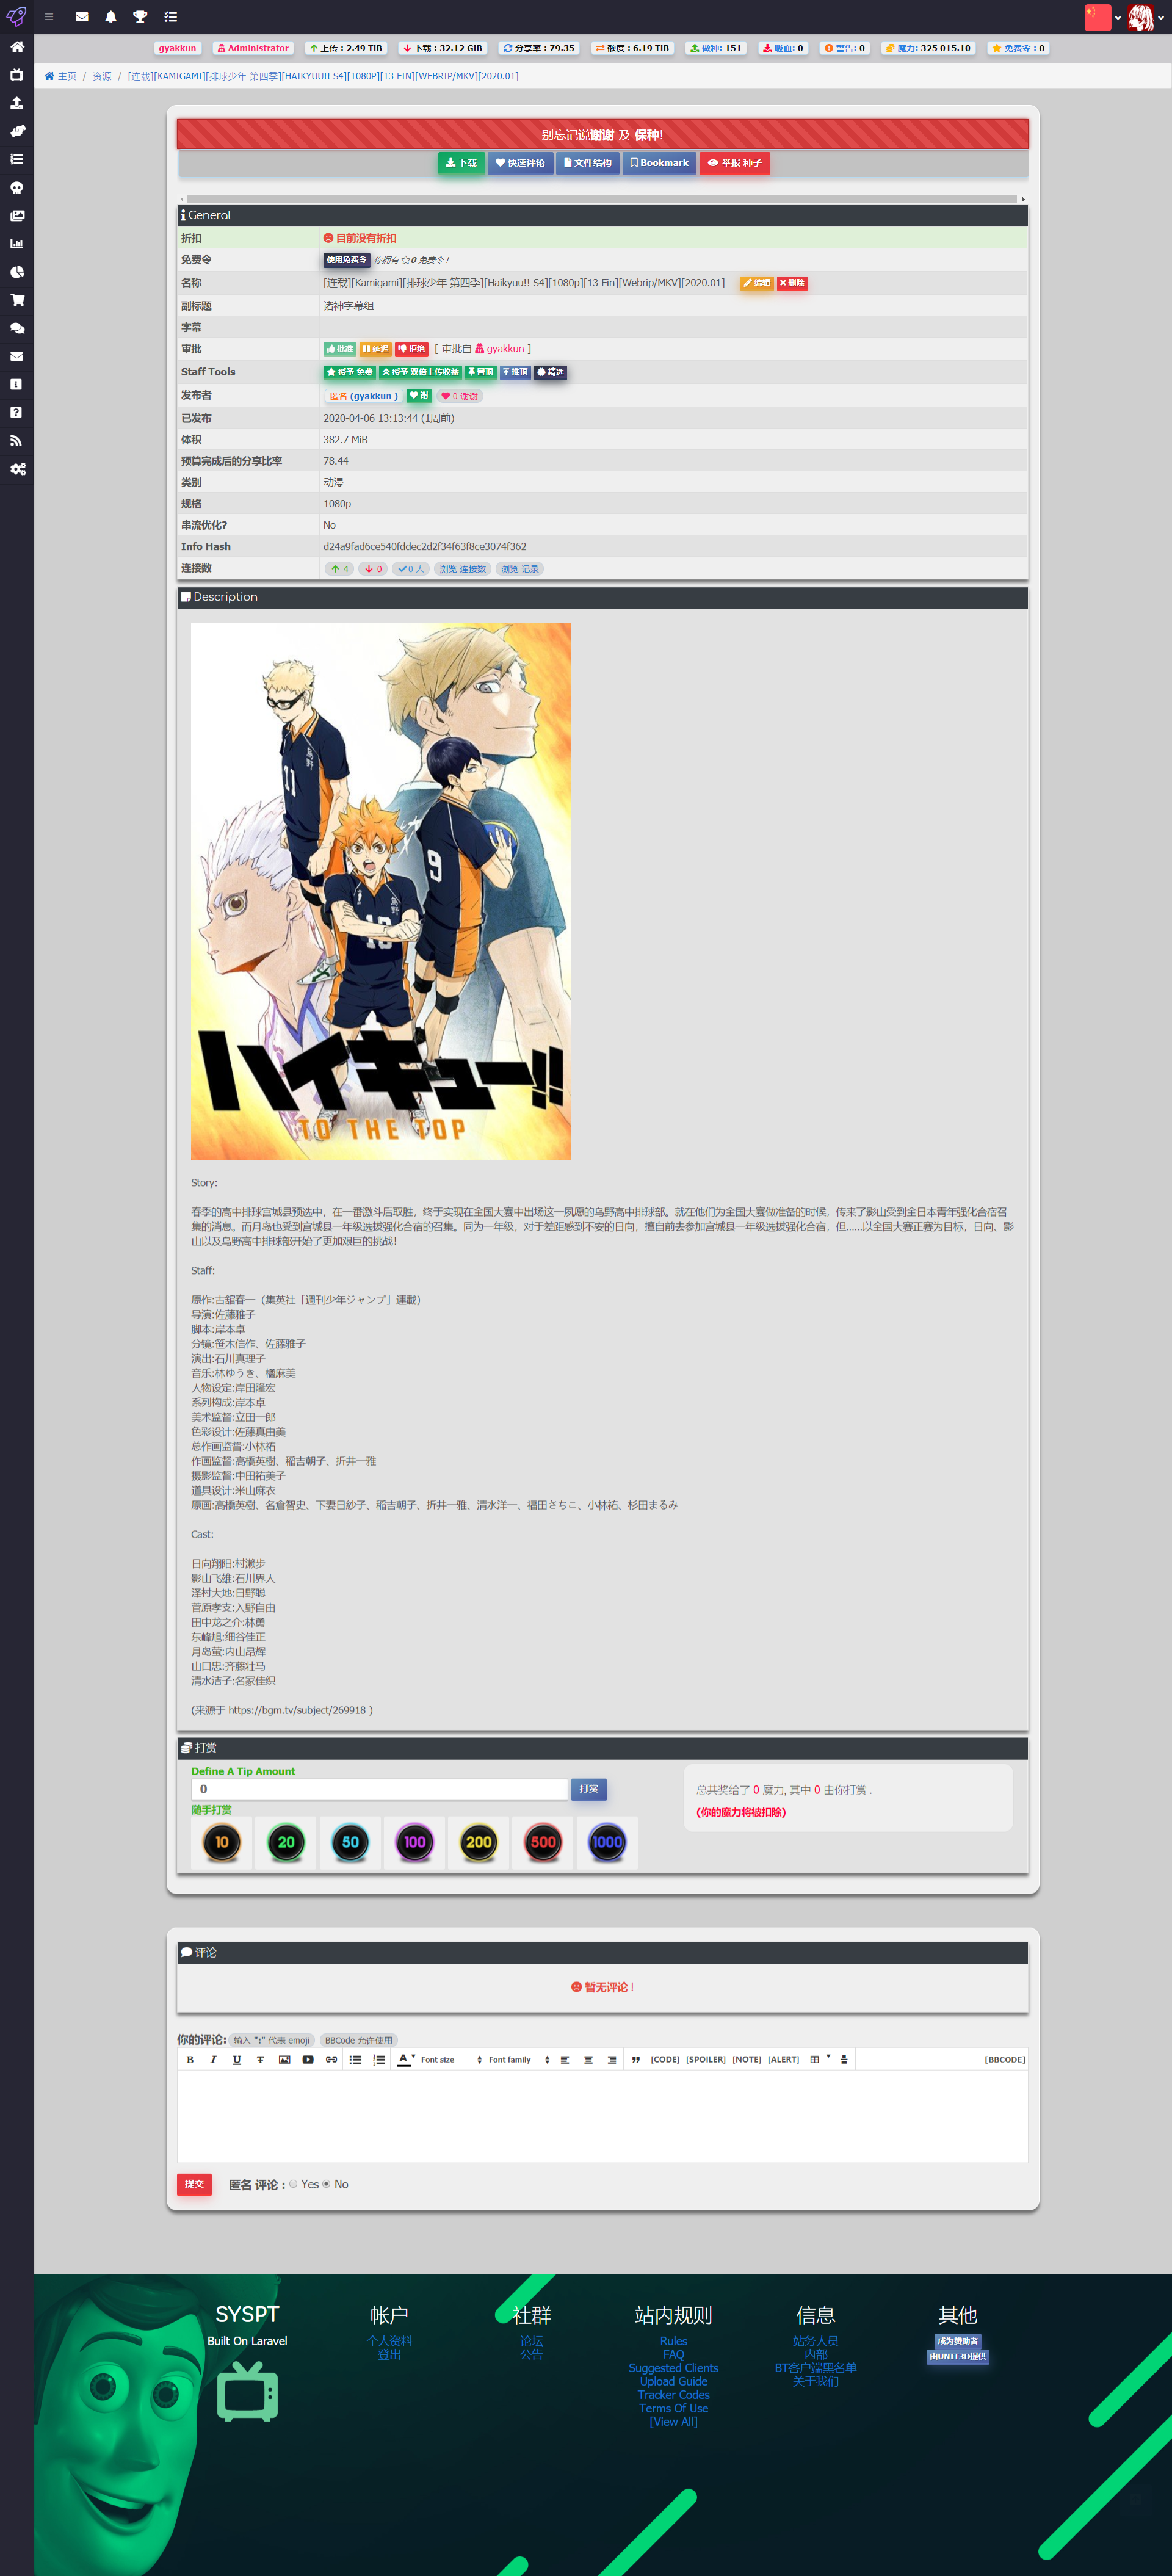
\includegraphics[width=0.65\textwidth]{support-files/5.2-torrent-detail-page.png}
    \caption{种子详情页}
    \label{fig:torrentdetailpage}
\end{figure}

\section{资源的发布}

点击页面左侧的资源发布图标, 进入资源发布页面。输入相应的种子描述信息后即可发布。注意到这里有原版中没有的副标题字段。

\begin{figure}[h]
    \centering
    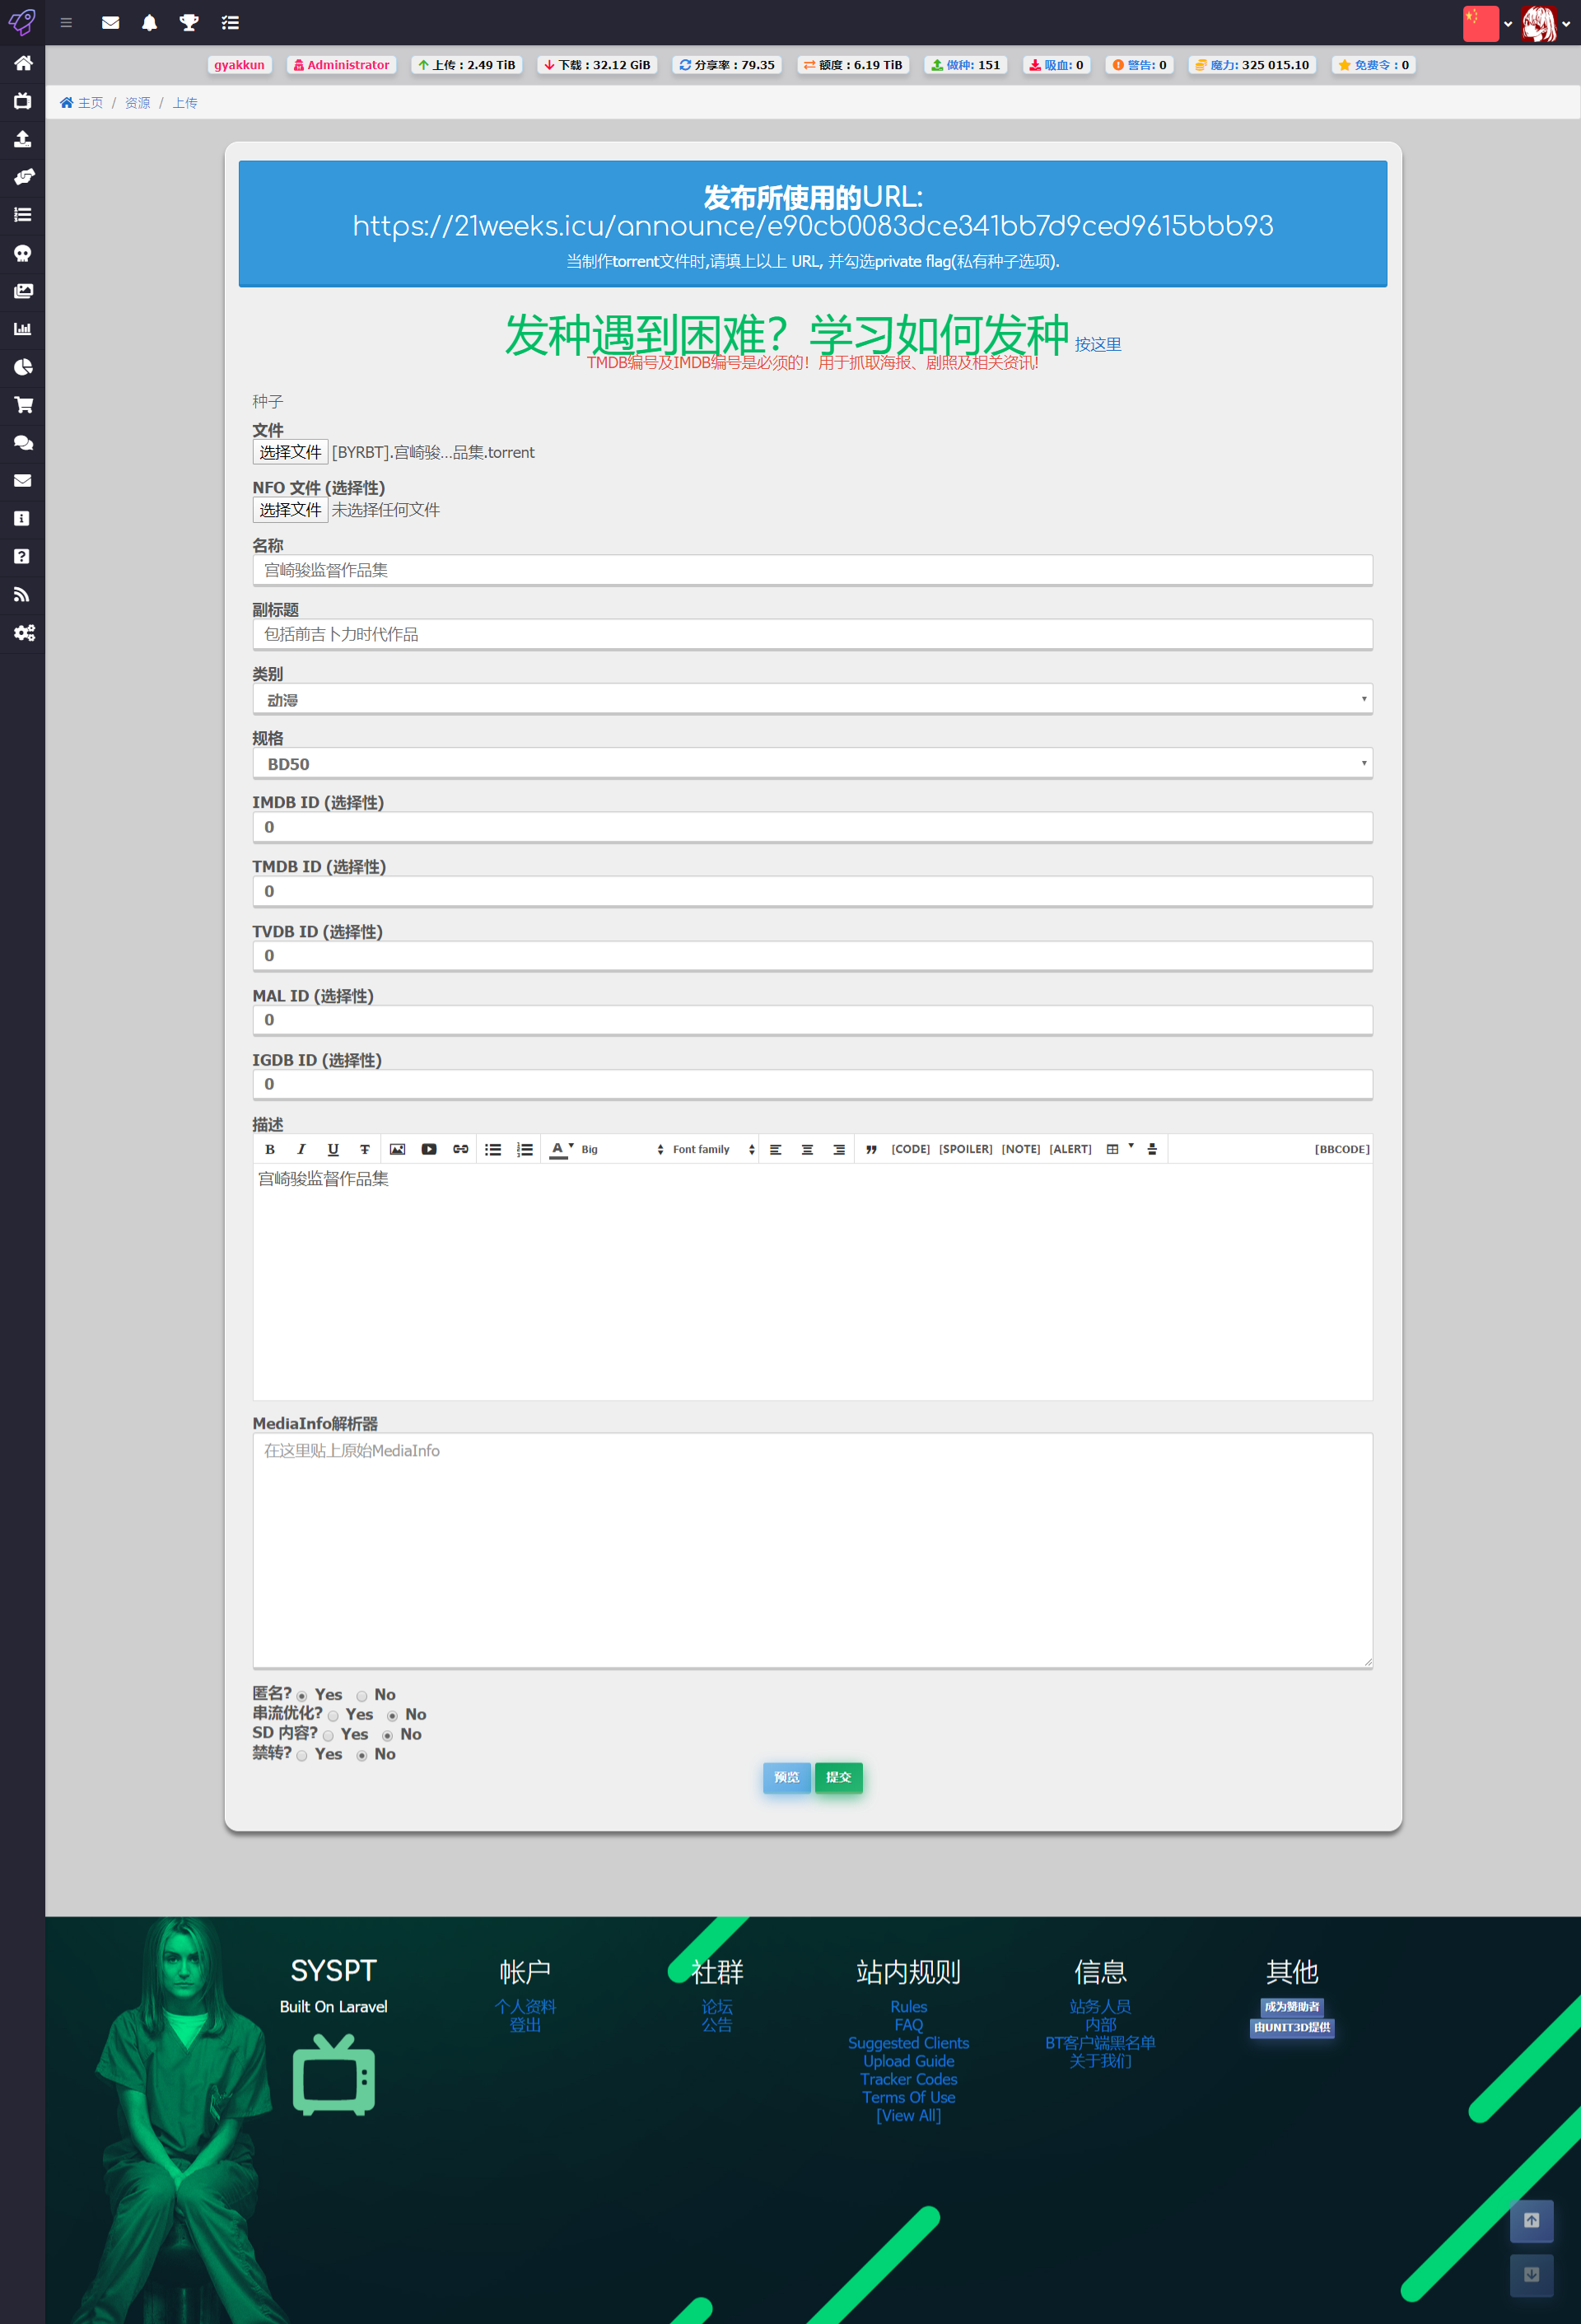
\includegraphics[width=0.75\textwidth]{support-files/5.2-upload-page.png}
    \caption{资源发布页}
    \label{fig:uploadpage}
\end{figure}

\newpage

\section{投票系统}

% 在管理员面板中可以发起投票

\begin{figure}[h]
    \centering
    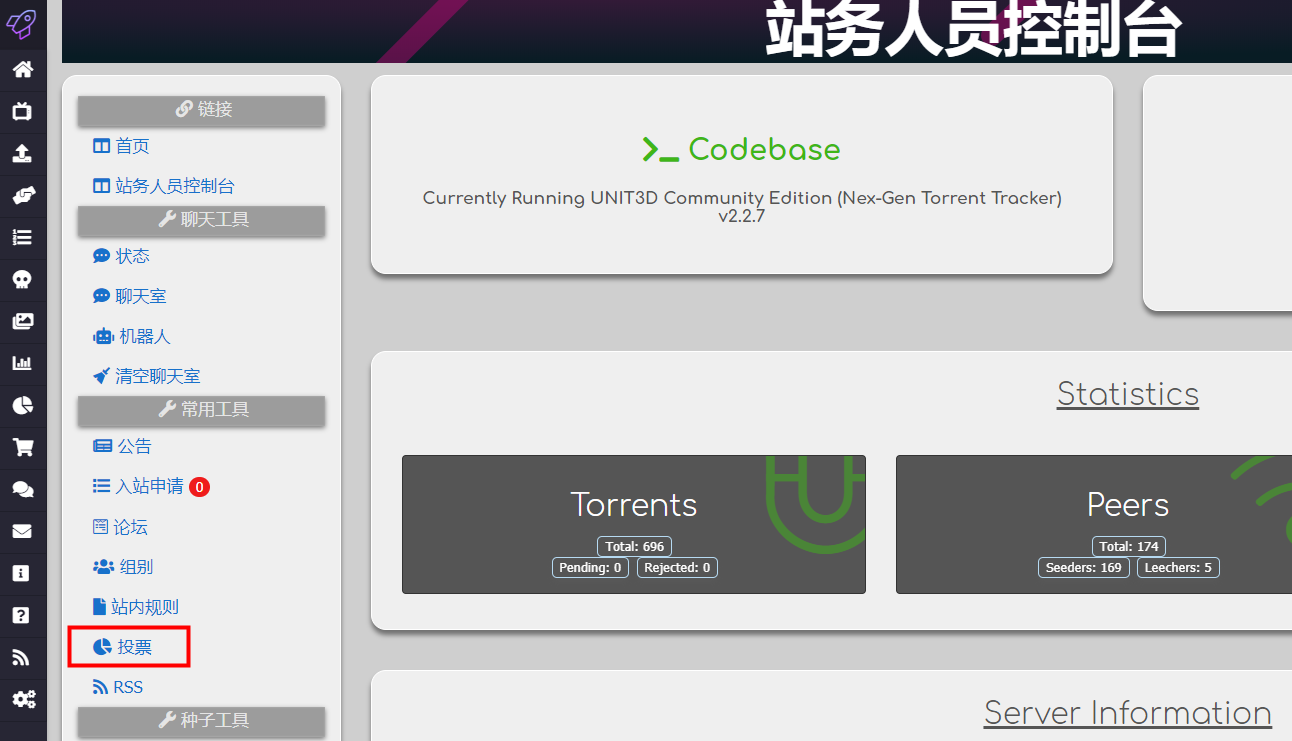
\includegraphics[width=0.8\textwidth]{support-files/5.x-poll-dashboard-entrance.png}
    \caption{管理员用的投票页入口}
    \label{fig:pollentrance}
\end{figure}

% \newpage

% 投票创建页

\begin{figure}[h]
    \centering
    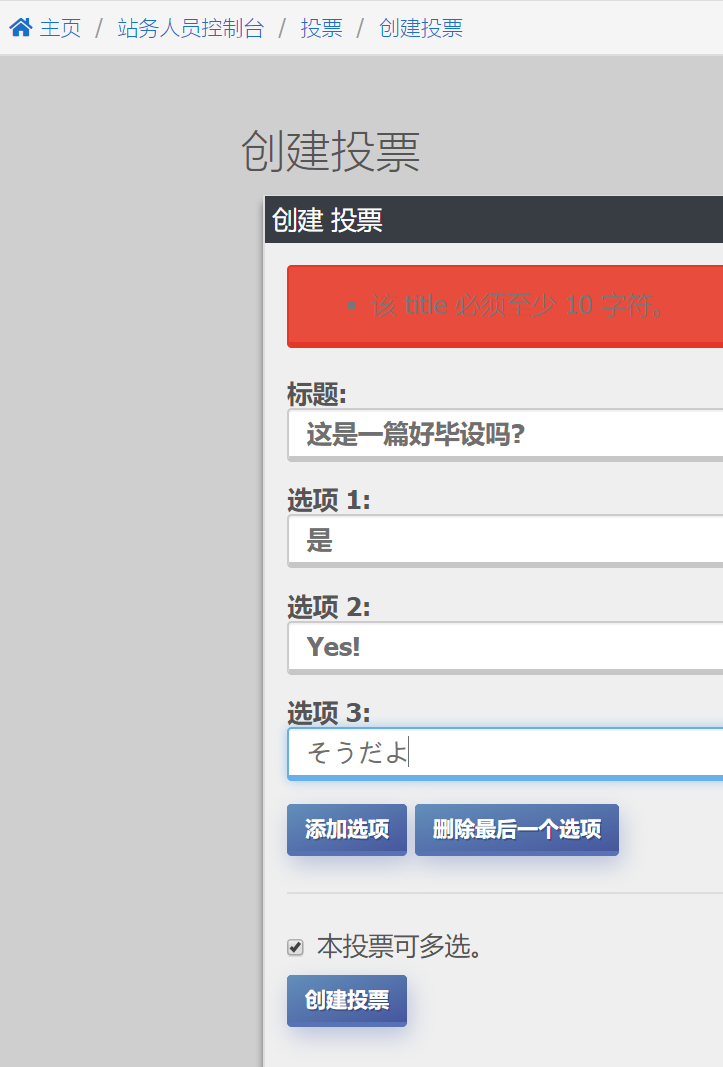
\includegraphics[width=0.45\textwidth]{support-files/5.x-poll-create-page-4.png}
    \caption{创建投票}
    \label{fig:createpoll}
\end{figure}

% \newpage

% 创建后可以在首页找到投票栏目

\begin{figure}[h]
    \centering
    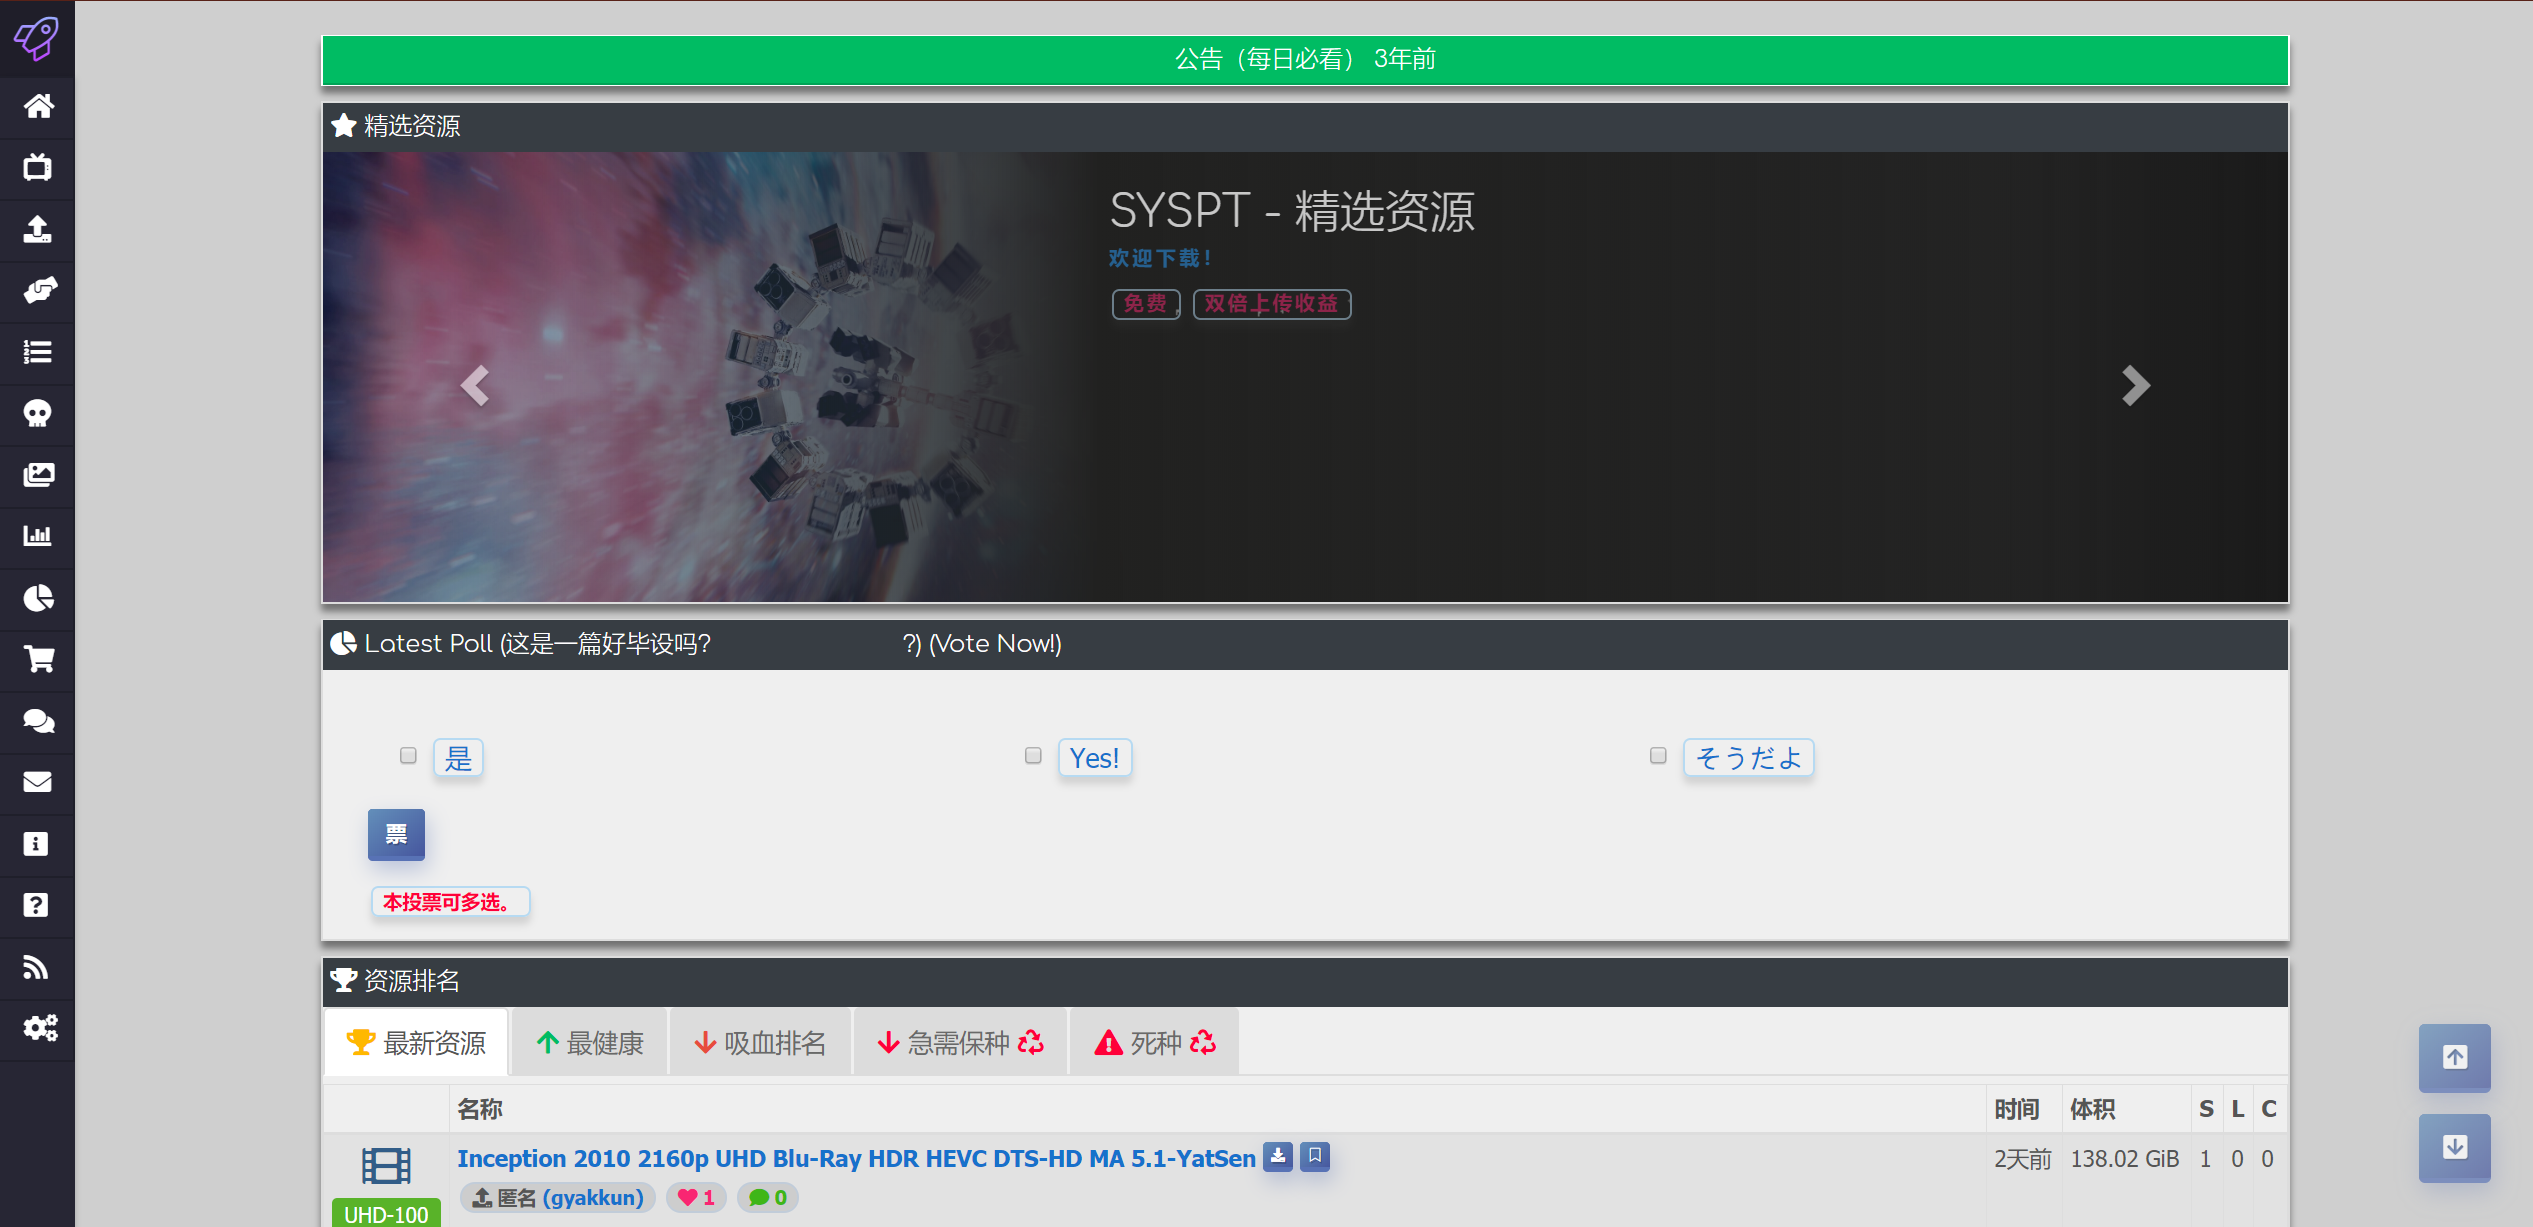
\includegraphics[width=0.8\textwidth]{support-files/5.x-poll-index-div.png}
    \caption{首页投票栏目}
    \label{fig:indexpoll}
\end{figure}

% \newpage

% 从左侧投票图标进入的投票列表页

\begin{figure}[h]
    \centering
    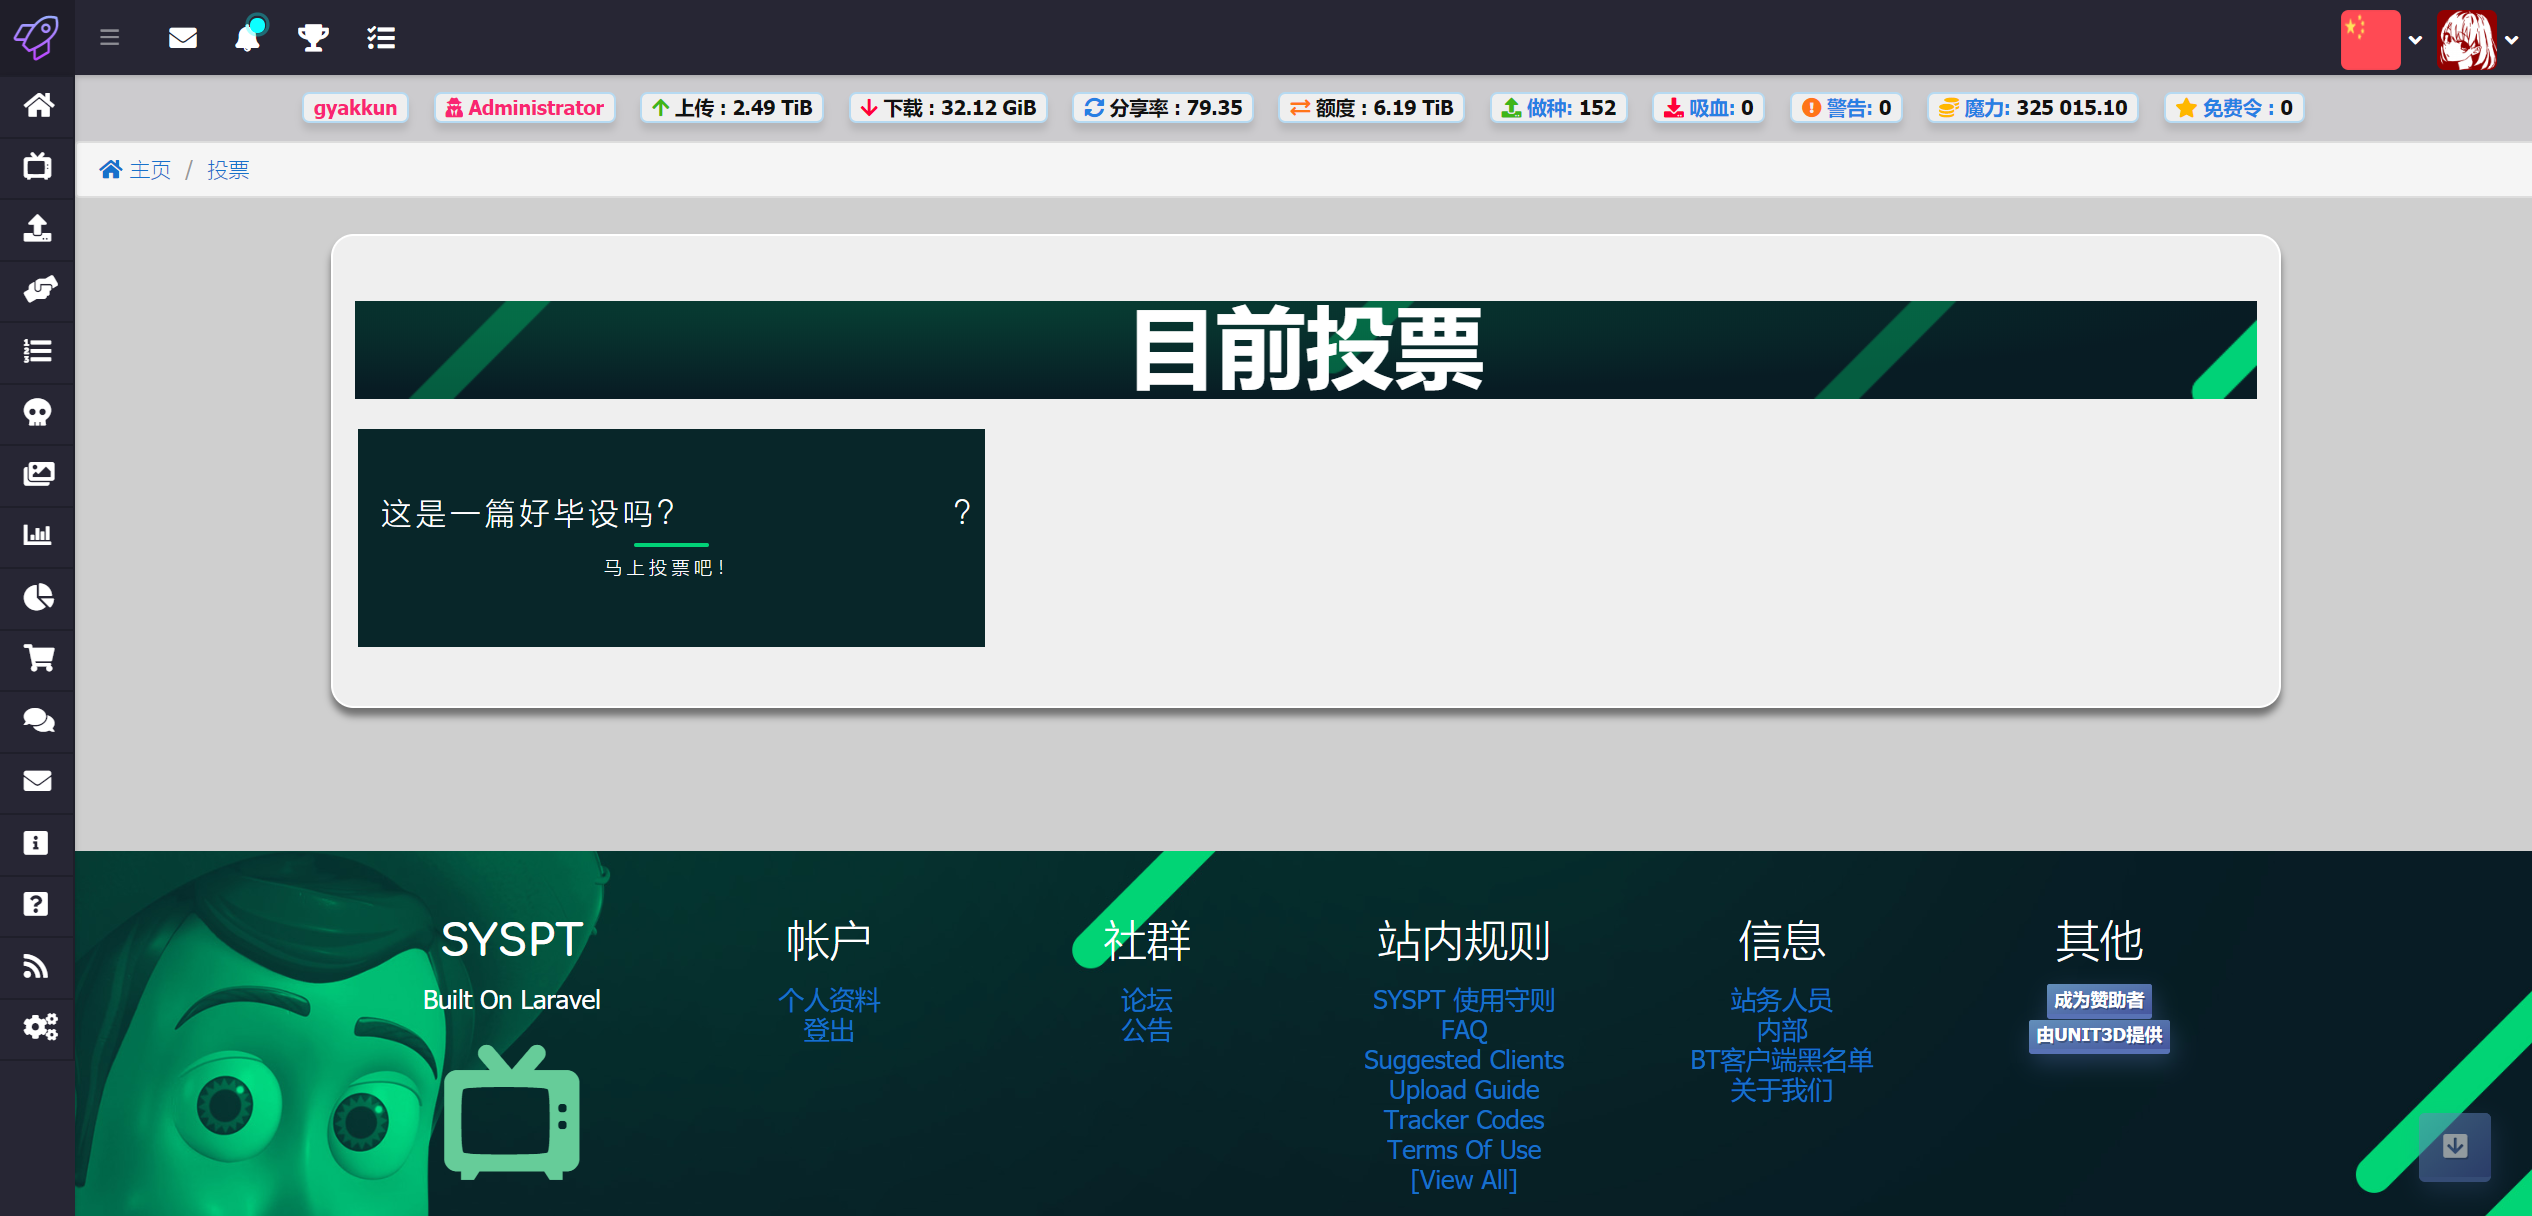
\includegraphics[width=0.8\textwidth]{support-files/5.x-poll-spec-page.png}
    \caption{从左侧投票徽标入口进入的投票列表页}
    \label{fig:leftnavpollentrance}
\end{figure}

% \newpage

% 具体一个投票的页面

\begin{figure}[h]
    \centering
    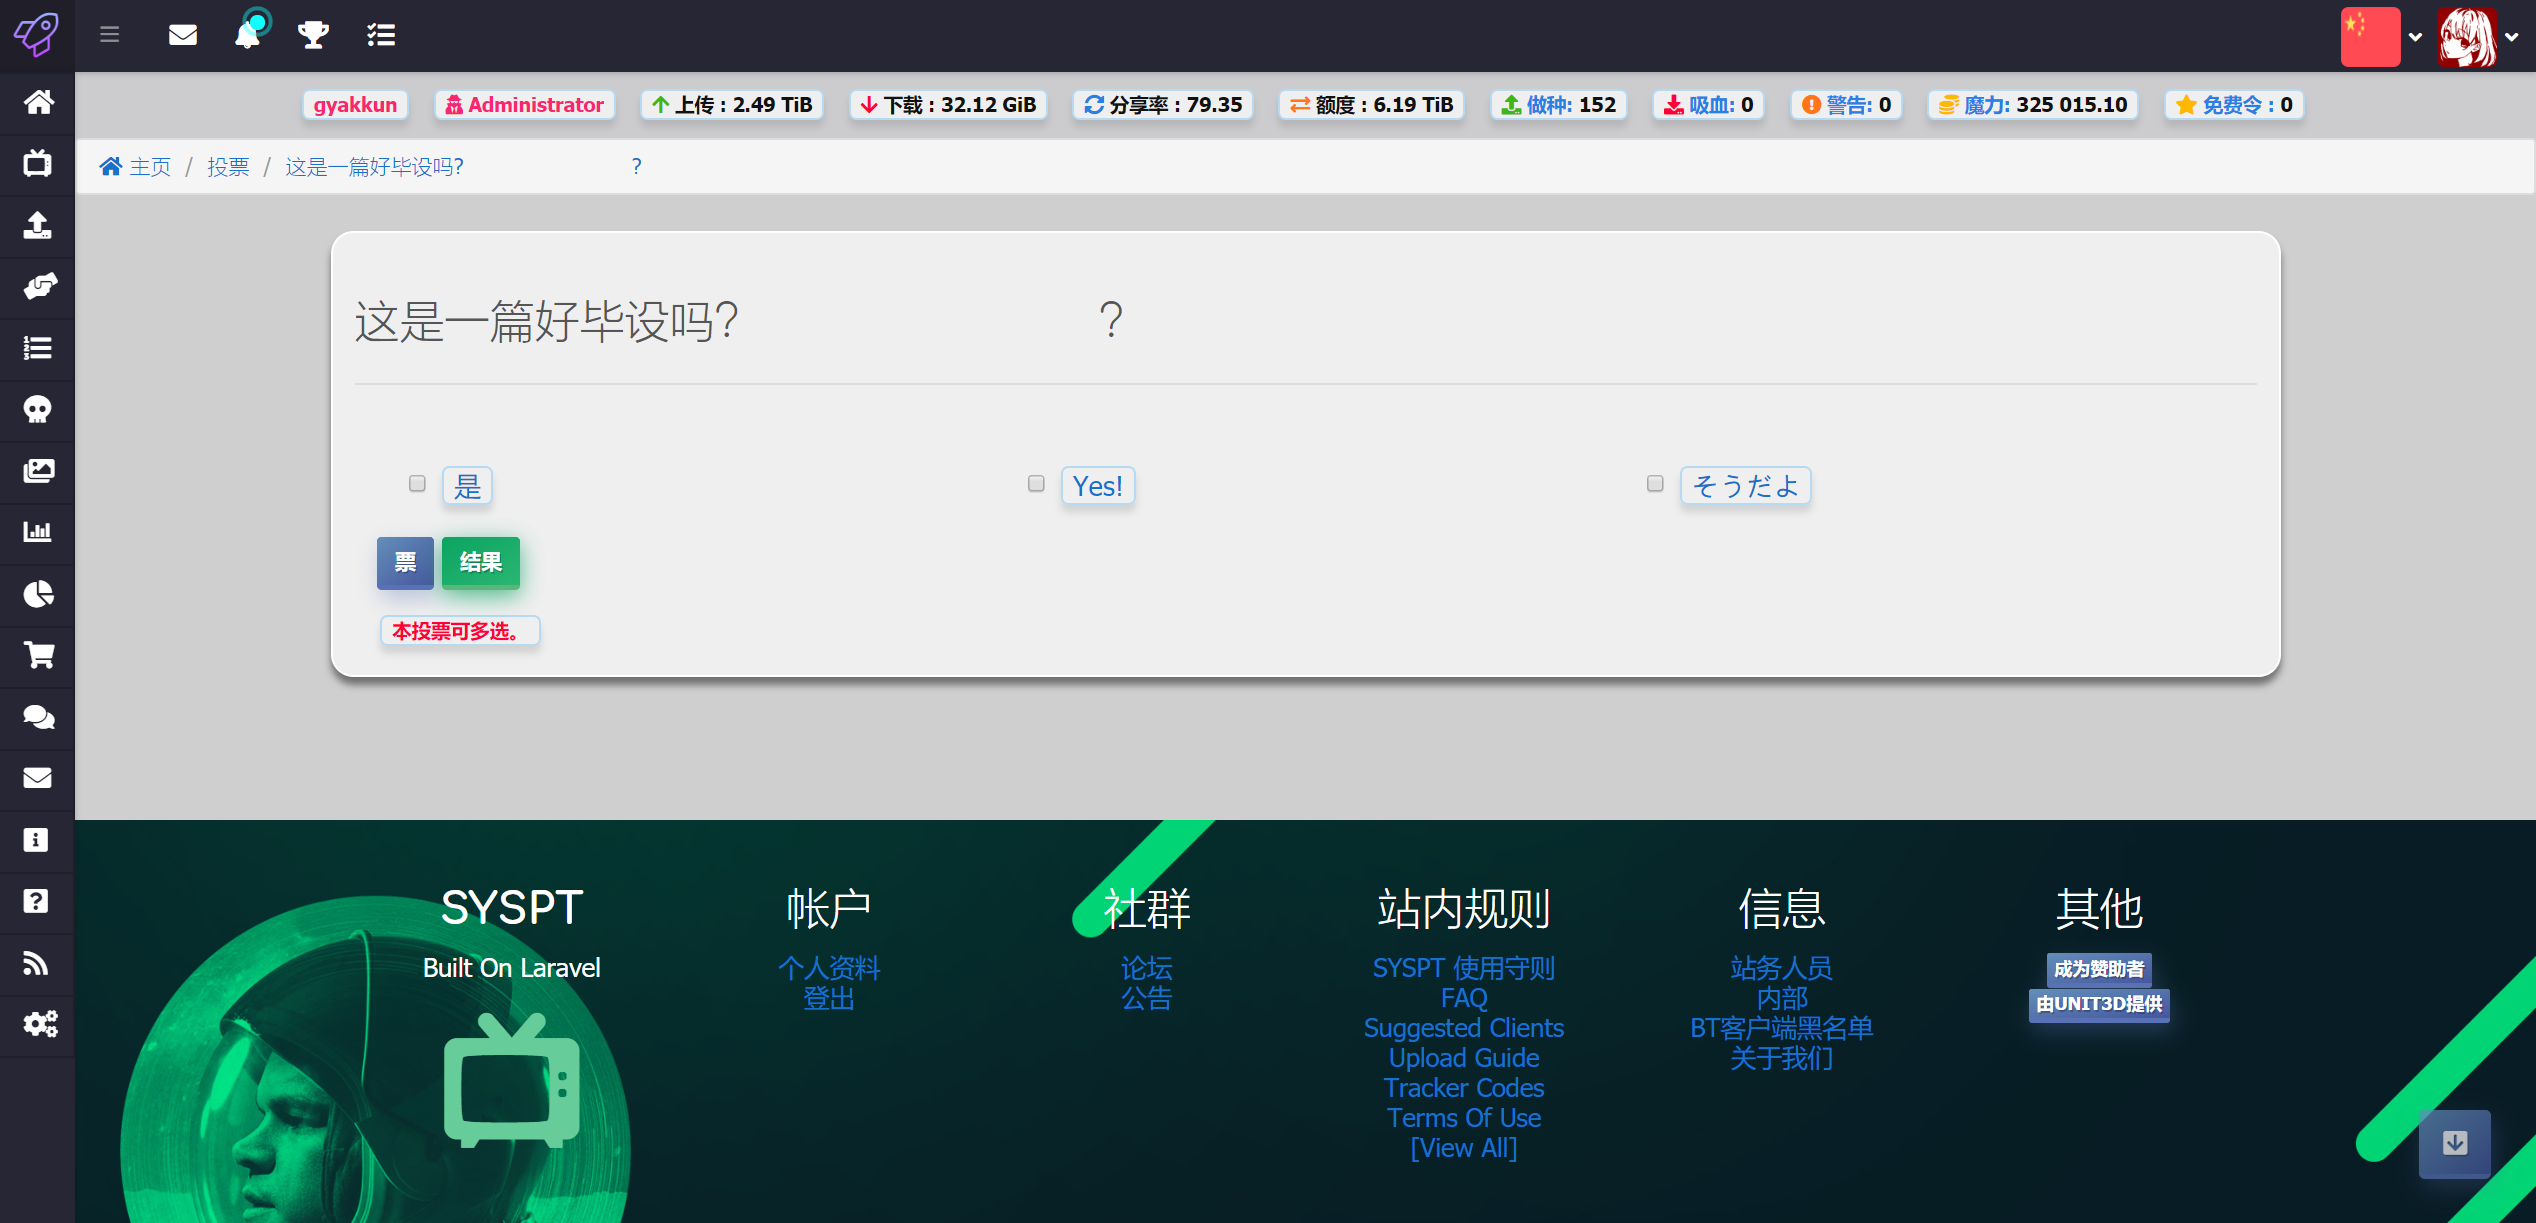
\includegraphics[width=0.8\textwidth]{support-files/5.x-poll-poll-page.png}
    \caption{具体投票页}
    \label{fig:pollpollpage}
\end{figure}

\section{BT客户端的使用}

种子文件下载到本地后, 使用BT客户端打开。如图所示为qBittorrent打开种子文件时弹出的窗口。

\begin{figure}[h]
    \centering
    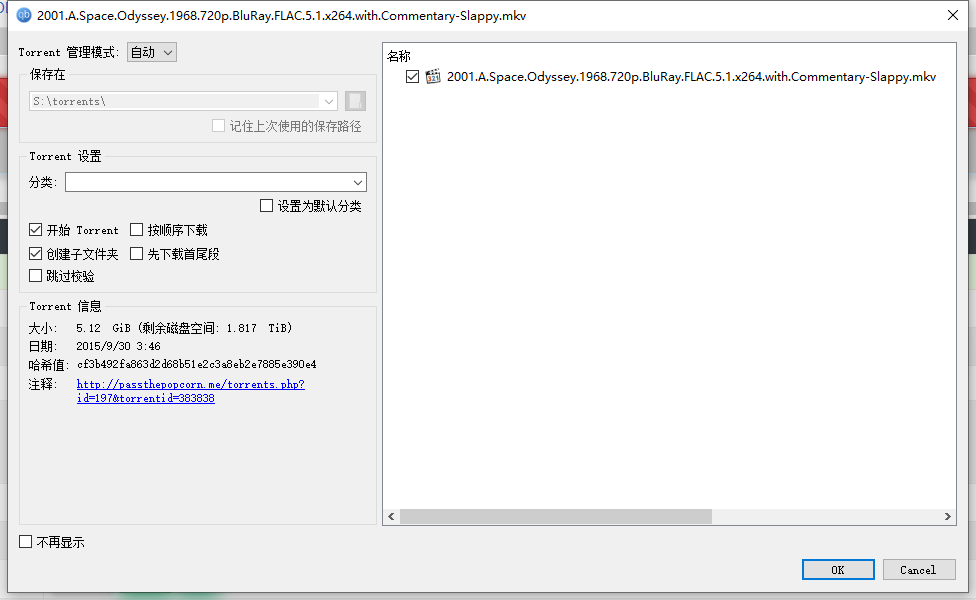
\includegraphics[width=0.65\textwidth]{support-files/5.4-bt-client-1.png}
    \caption{BT客户端 选择需要下载的文件}
    \label{fig:btclient1}
\end{figure}

